\documentclass[12pt,a4paper]{article}
\usepackage[UTF8]{ctex}
\usepackage{amsmath,amssymb}
\usepackage{xcolor}
\usepackage{hyperref}
\usepackage{geometry}
\usepackage{graphicx}
\geometry{margin=2.5cm}

\title{Quantum Boltzmann Machine / 量子玻尔兹曼机}
\author{QuoNic}
\date{}

\begin{document}
\maketitle

\begin{center}
\textbf{ML / 机器学习} | 难度：高级 | 预计时间：20 分钟
\end{center}

\tableofcontents
\newpage

\section{为什么需要？}

量子玻尔兹曼机是经典玻尔兹曼机的量子推广。

\subsection{经典局限}
\begin{itemize}
  \item 经典玻尔兹曼机训练慢
  \item 对于复杂分布，经典方法效率低
  \item 经典玻尔兹曼机容易陷入局部最优
\end{itemize}

\subsection{量子优势}
\begin{itemize}
  \item 量子玻尔兹曼机可以利用量子叠加和纠缠
  \item 训练速度更快
  \item 可以表示更复杂的分布
\end{itemize}

\subsection{实际应用}
\begin{itemize}
  \item 机器学习（生成模型）
  \item 优化（组合优化）
  \item 量子化学（分子模拟）
\end{itemize}

\section{快速上手}

\begin{verbatim}
from quonic.ml import qbm

# 训练量子玻尔兹曼机
data = [[0, 1], [1, 0], [1, 1], [0, 0]]
result = qbm(data=data, n_hidden=2)
print(f'Trained: {result.model}')
print(f'Loss: {result.loss}')
\end{verbatim}

\textbf{预期输出}：
\begin{verbatim}
Trained: QBM(n_visible=2, n_hidden=2)
Loss: 0.12
\end{verbatim}

\section{原理详解}

\subsection{电路图}

\begin{center}
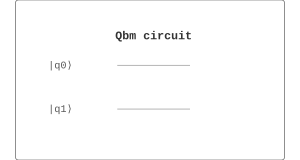
\includegraphics[width=0.6\textwidth]{../../images/qbm_circuit.svg}
\end{center}

\subsection{数学推导}

\textbf{Step 1: 量子玻尔兹曼机}

量子玻尔兹曼机：
\begin{equation}
\rho = \frac{e^{-\beta H}}{Z}
\end{equation}

其中 $H$ 是哈密顿量，$Z = \text{Tr}(e^{-\beta H})$ 是配分函数。

\textbf{Step 2: 哈密顿量}

哈密顿量：
\begin{equation}
H = \sum_i h_i Z_i + \sum_{ij} J_{ij} Z_i Z_j + \sum_i \Delta_i X_i
\end{equation}

\textbf{Step 3: 自由能}

自由能：
\begin{equation}
F = -\frac{1}{\beta} \ln Z
\end{equation}

\textbf{Step 4: 训练}

训练目标是最小化自由能：
\begin{equation}
\theta^* = \arg\min_\theta F(\theta)
\end{equation}

\textbf{Step 5: 梯度}

梯度：
\begin{equation}
\frac{\partial F}{\partial \theta_i} = \langle\frac{\partial H}{\partial \theta_i}\rangle_\rho
\end{equation}

\subsection{几何解释}

量子玻尔兹曼机在量子态空间中学习概率分布。量子叠加允许同时探索多个状态，量子纠缠允许表示复杂的关联。

\section{代码详解}

\begin{verbatim}
from quonic.ml import qbm

# qbm(data, n_hidden, n_epochs, learning_rate)
# data: 训练数据
# n_hidden: 隐藏单元数
# n_epochs: 训练轮数
# learning_rate: 学习率

result = qbm(
    data=[[0, 1], [1, 0], [1, 1], [0, 0]],
    n_hidden=2,
    n_epochs=100,
    learning_rate=0.01
)

# result.model: 训练后的模型
# result.loss: 损失值
# result.params: 参数
# result.history: 训练历史
print(f'Trained: {result.model}')
print(f'Loss: {result.loss}')
\end{verbatim}

\section{进阶用法}

\subsection{场景 1：不同隐藏单元数}

\begin{verbatim}
from quonic.ml import qbm

# 不同隐藏单元数
for n in [1, 2, 4, 8]:
    result = qbm(data=[[0,1],[1,0]], n_hidden=n)
    print(f'n={n}: Loss={result.loss}')
\end{verbatim}

\subsection{场景 2：不同数据}

\begin{verbatim}
from quonic.ml import qbm

# 不同数据
data1 = [[0, 1], [1, 0]]
data2 = [[0, 1, 0], [1, 0, 1], [1, 1, 0]]
data3 = [[0, 1, 0, 1], [1, 0, 1, 0], [1, 1, 0, 0]]

for data in [data1, data2, data3]:
    result = qbm(data=data, n_hidden=2)
    print(f'Loss: {result.loss}')
\end{verbatim}

\section{适用场景}

\subsection{机器学习}

量子玻尔兹曼机可以用于生成模型。

\subsection{优化}

量子玻尔兹曼机可以用于优化问题。

\subsection{量子化学}

量子玻尔兹曼机可以用于分子模拟。

\section{常见问题}

\subsection{量子玻尔兹曼机和经典玻尔兹曼机有什么区别？}

量子版本利用量子叠加和纠缠。

\subsection{量子玻尔兹曼机的训练速度如何？}

比经典版本更快。

\subsection{量子玻尔兹曼机需要多少量子比特？}

取决于可见单元和隐藏单元的数量。

\section{学习路径}

\subsection{前置知识}
\begin{itemize}
  \item 玻尔兹曼机
  \item 量子统计力学
  \item 量子机器学习
\end{itemize}

\subsection{继续学习}
\begin{itemize}
  \item 量子生成模型
  \item 量子优化
  \item 量子机器学习
\end{itemize}

\section{完整示例代码}

\subsection{示例 1：基本量子玻尔兹曼机}

\begin{verbatim}
from quonic.ml import qbm

result = qbm(data=[[0,1],[1,0]], n_hidden=2)
print(f'Trained: {result.model}')
\end{verbatim}

\section{下载}

\begin{itemize}
  \item [qbm.py](https://github.com/ChrisLee0721/QuoNic/blob/main/examples/qbm/qbm.py)
\end{itemize}

\end{document}
